\documentclass{article}
\usepackage{graphicx} % Required for inserting images
\usepackage{amssymb}
\usepackage{amsmath}
\usepackage{setspace}
\usepackage{ulem}
\usepackage[top=2cm,bottom=2cm,left=2.5cm,right=2.5cm,marginparwidth=1.5cm]{geometry}

% Roman Numbers, \rmnum{} & \Rmnum{}
\makeatletter
\newcommand{\rmnum}[1]{\romannumeral #1}
\newcommand{\Rmnum}[1]{\expandafter\@slowromancap\romannumeral #1@}

\title{CSCI-SHU 360 Homework1}
\author{Ninghao Lu nl2752}
\date{2024 Fall}

\begin{document}

\maketitle

\section*{Exercise 1 Simpson's Paradox}
\subsection*{1.1 Solution:}
\subsubsection*{For machine 1:}
Let $A_1$ denote the event that I win on machine 1, my winning probability is 
\begin{align*}
    P(A_1) = \frac{40}{40 + 60} = \frac{40}{100} = 0.4
\end{align*}
Let $B_1$ denote the event that my friend wins on machine 1, the winning probability is 
\begin{align*}
    P(B_1) = \frac{30}{30 + 70} = \frac{30}{100} = 0.3
\end{align*}
Since 0.4 $>$ 0.3, we have $P(A_1) > P(B_1)$, I am more likely to win on machine 1.
\subsubsection*{For machine 2:}
Let $A_2$ denote the event that I win on machine 2, my winning probability is 
\begin{align*}
    P(A_2) = \frac{210}{210 + 830} = \frac{210}{1040} = \frac{21}{104}
\end{align*}
Let $B_2$ denote the event that my friend wins on machine 2, the winning probability is 
\begin{align*}
    P(B_2) = \frac{14}{14 + 70} = \frac{14}{84} = \frac{1}{6}
\end{align*}
Since $\frac{21}{104} > \frac{1}{6}$, we have $P(A_2) > P(B_2)$, I am more likely to win on machine 2.\\
In conclusion, I am more likely to win on both machines.

\subsection*{1.2 Solution:}
Let $A$ denote the event that I win on both machines and let B denote the event that my friend wins on both machines.
\begin{align*}
    P (A) &= \frac{\text{Number of wins}}{\text{Number of trials}} = \frac{40 + 210}{40 + 60 + 210 + 830} = \frac{250}{1140} = \frac{25}{114} \\
    P (B) &= \frac{\text{Number of wins}}{\text{Number of trials}} = \frac{30 + 14}{30 + 70 + 14 + 70} = \frac{44}{184} = \frac{11}{46} 
\end{align*} 
Since $\frac{25}{114} > \frac{11}{46}$, we have $P(A) < P(B)$, my friend is more likely to win. 

\subsection*{1.3 Solution:}
Let $M_1$ denote the event that I play on machine 1, $M_2$ denote the event that I play on the second machine. Let $N_1$ denote the event that my friend plays on machine 1, $N_2$ denote the event that my friend plays on the second machine. \\
My winning probability is
\begin{align*}
    P(A) &= P(A \cap M_1) + P(A \cap M_2) = P(A | M_1) P(M_1) + P(A | M_2) P(M_2) \\
         &= \frac{2}{5} \cdot \frac{100}{100 + 1040} + \frac{21}{104} \cdot \frac{1040}{100 + 1040} = \frac{2}{5} \cdot \frac{100}{1140} + \frac{21}{104} \cdot \frac{1040}{1140} \\
         &= \frac{4}{114} + \frac{21}{114} \\
         &= \frac{25}{114}
\end{align*}
My friend's winning probability is
\begin{align*}
    P(B) &= P(B \cap N_1) + P(A \cap N_2) = P(B | N_1) P(N_1) + P(B | N_2) P(N_2) \\
         &= \frac{3}{7} \cdot \frac{100}{100 + 84} + \frac{14}{84} \cdot \frac{84}{100 + 84} = \frac{3}{10} \cdot \frac{100}{184} + \frac{1}{6} \cdot \frac{84}{184} \\
         &= \frac{30}{184} + \frac{14}{184} \\
         &= \frac{11}{46}
\end{align*}
From the above computing process we can see the the overall probability is affected by both the probability on each machine and the fraction of the number of trails on each machine. Although my winning probability is higher on each machine, I conduct more much trials on machine 2 and my winning probability on is lower than that on machine 1, which lowers my overall probability.

\section*{Exercise 2 Matrix as operations}
\subsection*{2.1 Solution:}
We want to find a matrix $W$ that transforms $a_1$ to $b_1$ and $a_2$ to $b_2$.
Let
\[
\begin{bmatrix} w_{11} & w_{12} \\ w_{21} & w_{22} \end{bmatrix} \begin{bmatrix} 1 \\ 1 \end{bmatrix} = \begin{bmatrix} -0.8 & 1.6 \end{bmatrix}
\]
\[
\begin{bmatrix} w_{11} & w_{12} \\ w_{21} & w_{22} \end{bmatrix} \begin{bmatrix} 1 \\ -1 \end{bmatrix} = \begin{bmatrix} 2.6 & -0.2 \end{bmatrix}
\]
Hence,
\[
\begin{bmatrix} w_{11} + w_{12} \\ w_{21} + w_{22} \end{bmatrix} = \begin{bmatrix} -0.8 \\ 1.6 \end{bmatrix}
\]
\[
\begin{bmatrix} w_{11} - w_{12} \\ w_{21} - w_{22} \end{bmatrix} = \begin{bmatrix} 2.6 \\ -0.2 \end{bmatrix}
\]
Solving the equations, we have
\begin{align*}
    w_{11} = 0.9 \quad w_{12} = -1.7 \quad w_{21} = 0.7 \quad w_{22} = 0.9
\end{align*}
In conclusion, 
\begin{align*}
    W = \begin{bmatrix} 0.9 & -1.7 \\ 0.7 & 0.9 \end{bmatrix}
\end{align*}

\subsection*{2.2 Solution}
% V
For a matrix V which rotates clockwise by $\alpha$ degrees, we assume it to be
\[
\begin{bmatrix} cos \alpha & sin \alpha \\ -sin \alpha & cos \alpha \end{bmatrix} 
\]
Since tan$\alpha$ = 3, suppose $\alpha \in [0,180^\circ]$, we have sin$\alpha = \frac{3}{\sqrt{10}}$, cos$\alpha = \frac{1}{\sqrt{10}}$. As a result, 
\[
V = \begin{bmatrix} \frac{1}{\sqrt{10}} & \frac{3}{\sqrt{10}} \\ -\frac{3}{\sqrt{10}} & \frac{1}{\sqrt{10}} \end{bmatrix} 
\]

% \Sigma
For a matrix $\Sigma$ which scales the y-axis by 2, while keeps the x-axis unchanged, let $x = \begin{bmatrix} a \\ b \end{bmatrix}$, with a, b $\in \mathbb{R}$
\[
    \Sigma x = \begin{bmatrix} \Sigma_{11} & \Sigma_{12} \\ \Sigma_{21} & \Sigma_{22} \end{bmatrix} x = \begin{bmatrix} a \Sigma_{11} + b \Sigma_{12} \\ a \Sigma_{21} + b \Sigma_{22} \end{bmatrix} = \begin{bmatrix} a \\ 2b\end{bmatrix}
\]
Hence, we can take $\Sigma_{11} = 1, \Sigma_{12} = 0, \Sigma_{21} = 0, \Sigma_{22} = 2$ and 
\[
\Sigma = \begin{bmatrix} 1 & 0 \\ 0 & 2 \end{bmatrix} 
\]

% U
For a matrix U which rotates counter-clockwise by $\beta$ degrees, we assume it to be
\[
\begin{bmatrix} cos \beta & -sin \beta \\ sin \beta & cos \beta \end{bmatrix} 
\]
Since tan$\beta = \frac{1}{3}$, suppose $\beta \in [0,180^\circ]$, we have sin$\beta = \frac{1}{\sqrt{10}}$, cos$\beta = \frac{3}{\sqrt{10}}$. As a result, 
\[
U = \begin{bmatrix} \frac{3}{\sqrt{10}} & -\frac{1}{\sqrt{10}} \\ \frac{1}{\sqrt{10}} & \frac{3}{\sqrt{10}} \end{bmatrix} 
\]

% U\SigmaV
Therefore,
\[
U \Sigma V = \begin{bmatrix} \frac{3}{\sqrt{10}} & -\frac{1}{\sqrt{10}} \\ \frac{1}{\sqrt{10}} & \frac{3}{\sqrt{10}} \end{bmatrix} \begin{bmatrix} 1 & 0 \\ 0 & 2 \end{bmatrix} \begin{bmatrix} \frac{1}{\sqrt{10}} & \frac{3}{\sqrt{10}} \\ -\frac{3}{\sqrt{10}} & \frac{1}{\sqrt{10}} \end{bmatrix}
\]
\[
= \begin{bmatrix} \frac{3}{\sqrt{10}} & -\frac{1}{\sqrt{10}} \\ \frac{1}{\sqrt{10}} & \frac{3}{\sqrt{10}} \end{bmatrix} \begin{bmatrix} \frac{1}{\sqrt{10}} & \frac{3}{\sqrt{10}} \\ -\frac{6}{\sqrt{10}} & \frac{2}{\sqrt{10}} \end{bmatrix}
\]
\[
= \begin{bmatrix} \frac{9}{10} & \frac{7}{10} \\ -\frac{17}{10} & \frac{9}{10} \end{bmatrix} = \begin{bmatrix} 0.9 & 0.7 \\ -1.7 & 0.9 \end{bmatrix}
\]
We could discover that $U \Sigma V = W^T$

\subsection*{2.3 Solution}
\subsubsection*{Compute eigenvalues and eigenvectors}
\[
W^T W = \begin{bmatrix} \frac{9}{10} & \frac{7}{10} \\ -\frac{17}{10} & \frac{9}{10} \end{bmatrix} \begin{bmatrix} \frac{9}{10} & -\frac{17}{10} \\ \frac{7}{10} & \frac{9}{10} \end{bmatrix} = \begin{bmatrix} \frac{13}{10} & -\frac{9}{10} \\ -\frac{9}{10} & \frac{37}{10} \end{bmatrix}
\]
To compute the eigenvalues and eigenvectors, the characteristic equation is 
\begin{align*}
    det(W^T W - \lambda I) &= 0 \\
    (1.3 - \lambda)(3.7 - \lambda) - 0.81 &= 0 \\
    \lambda ^ 2 - 5 \lambda + 4 &= 0 \\
    (\lambda - 4)(\lambda - 1) &= 0
\end{align*}
Therefore, the eigenvalues are $\lambda = 1$ and $\lambda = 4$. \\
For $\lambda = 1$, 
\begin{align*}
    W^T W - \lambda I &= W^T W - I = \begin{bmatrix} 0.3 & -0.9 \\ -0.9 & 2.7 \end{bmatrix}
\end{align*}

We have, $(W^T W - I)x = 0$, which is
\[
\begin{bmatrix} 0.3 & -0.9 \\ -0.9 & 2.7 \end{bmatrix} x = 0
\]
So $x$ can be $\begin{bmatrix} 3 \\ 1 \end{bmatrix}$.

For $\lambda = 4$, 
\begin{align*}
    W^T W - \lambda I &= W^T W - 4I = \begin{bmatrix} -2.7 & -0.9 \\ -0.9 & -0.3 \end{bmatrix}
\end{align*}

We have, $(W^T W - 4I)x = 0$, which is
\[
\begin{bmatrix} -2.7 & -0.9 \\ -0.9 & -0.3 \end{bmatrix} x = 0
\]
So $x$ can be $\begin{bmatrix} 1 \\ -3 \end{bmatrix}$.

For $\lambda = 1$, its corresponding eigenvector is $\begin{bmatrix} 3 \\ 1 \end{bmatrix}$; for $\lambda = 4$, its corresponding eigenvector is $\begin{bmatrix} 1 \\ -3 \end{bmatrix}$. 
\subsubsection*{Shape after transformation}
Suppose every point on the unit circle gets transformed by W, we will get an ellipse after the transformation. This is because transforming by W is equivalent to transforming by $U \Sigma V$ according to previous question. This is a process that first rotates each point (still get a circle), then scaling (resulting in an ellipse), and finally rotating the ellipse.
\subsubsection*{Relationship between transformed shape and eigenvalues and eigenvectors}
The eigenvalues corresponds to squared length of the semi-major and semi-minor of the ellipse. And the eigenvectors indicate the directions of the axes. \\
\uline{Explanation:}\\
Since U and V are orthonormal matrix, and $\Sigma$ is symmetric, for a vector $x = \begin{bmatrix} x_1 \\ x_2 \end{bmatrix}$ which is on the unit circle, we have
\[
x^T x = 1
\]
because for any point on the unit cricle its coordinates satisfies $x_1^2 + x_2^2 = 1$. Since $W^T = U \Sigma V$, after transformation by W, we have
\begin{align*}
    (W x)^T W x &= x^T W^T W x = x^T (U \Sigma V)(U \Sigma V)^T x \\
                &= x^T U \Sigma V V^T \Sigma U^T x \\
                &= x^T U \Sigma^2 U^T x \\
\end{align*}
Here we let y = $U^T x$, where $y^T y = (U^T x)^T (U^T x) = x^T x = 1$, and the equation above becomes
\newpage
\begin{align*}
    x^T U \Sigma^2 U^T x &= y^T \Sigma^2 y \\
                         &= \sum_{i=1}^{2} \sigma_i^2 y_i^2 \\
                         &= \sigma_1^2 y_1^2 + \sigma_2^2 y_2^2
\end{align*}
where  $\sigma_1, \sigma_2$ are elements on the diagonal of matrix $\Sigma$. And we assume 
\[
\sigma_1^2 y_1^2 + \sigma_2^2 y_2^2 = k, \ k \in \mathbb{R}
\]
From this equation, we can see that the original equation of a unit circle  $x_1^2 + x_2^2 = 1$ is transformed into an equation for an ellipse. The semi-major and semi-minor of the ellipse is $\sigma_1^2, \sigma_2^2$.
\textbf{It is quite obvious that eigenvalues corresponds to squared length of the semi-major and semi-minor of the ellipse since the eigenvalues of $W^T W$ is $\sigma_1^2, \sigma_2^2$.}\\
For the unit circle, the direction of the axes can be indicated by $v_1 = \begin{bmatrix} 1 \\ 0 \end{bmatrix}$ and $v_2 = \begin{bmatrix} 0 \\ 1 \end{bmatrix}$.
For the current ellipse, the direction of the axes after transformation can be indicated by $c_1 = U^T v_1$ and $c_2 = U^T v_2$. Since U is a $2 \times 2$ rotation matrix, the eigenvector of $U^T$ and U are the same. \textbf{It is also obvious that the eigenvectors indicate the directions of the axes since the eigenvectors of $W^T W$ are columns of U.}
 






% \begin{align*}
%     W^T W &= (U \Sigma V) ( U \Sigma V)^T  \\
%               &= U \Sigma V V^T \Sigma^T U^T= U \Sigma^T \Sigma U^T = U \Sigma^2 U^T
% \end{align*}
% We can see that this is actually a diagonalization of $W^T W$ where the elements on the main diagonal of ($\Sigma^T \Sigma$) are eigenvalues and columns of U are corresponding eigenvectors. \\
% The elements on the main diagonal of ($\Sigma ^T \Sigma$) are squares of elements on the main diagonal of $\Sigma$ (singular values). However, since the effect of $\Sigma$ is scaling and its singular values corresponds to the length of semi-major/minors, we can conclude that the eigenvalues of ($\Sigma^T \Sigma$) corresponds to the squares of the lengths of semi-major/minors of the ellipse.\\
% Moreover, since the rotation of the axes of the ellipse is obtained by U, which means mapping the original coordinate system into another system spanned by columns of U, and the eigenvectors of ($W^T W$) are U's columns, we can infer that the eigenvectors of $W^T W$ can indicate the directions of the ellipse's axes.

\subsection*{2.4 Solution}
The determinant of W is
\begin{align*}
    det(W) = det \begin{bmatrix} 0.9 & -1.7 \\ 0.7 & 0.9 \end{bmatrix} = 0.81 + 1.19 = 2
\end{align*}
The area of the ellipse is $S_{ellipse} = 2 \cdot 1 \cdot \pi = 2 \pi$, which is equal to the determinant of W $\cdot$ \{Area of the unit circle\}. So the relationship between the determinant and the area of a transformed shape is that: \\
the absolute value of determinant is the fraction between the area of the transformed shape and the area of the original shape. \\
Based on that, one simple explanation for $det(AB) = det(A) det(B)$ is transforming a shape by AB is equivalent to conduct the transformation with A first and then B, and the scaling effect of AB is equivalent to the cumulative scaling effect of A and B.


\section*{Exercise 3 Some practices}
\subsection*{3.1 Solution}
Let a discrete random variable Y = $X^e$, its variance can be written as
\begin{align*}
    Var(Y) = E[Y^2] - (E[Y])^2 = E[(X^3)^2] - (E[X^3])^2
\end{align*}
Since Var(Y) $\geq$ 0, we have $E[(X^3)^2] - (E[X^3])^2 \geq 0$. Therefore, $(E[X^3])^2 \leq E[X^6]$.

\subsection*{3.2 Solution}
We can proceed by Cauchy-Schwarz Inequality, which states that for any two random variables A and B, 
\begin{align*}
    (E[AB])^2 \leq E[A^2]E[B^2]
\end{align*}
Applying this inequality here, we let A = $X^3$, B = 1 and we have
\begin{align*}
    (E[X^3])^2 \leq E[(X^3)^2]E[1] = E[X^6]E[1] = E[X^6]
\end{align*}
Therefore, we can conclude that $(E[X^3])^2 \leq E[X^6]$.

\subsection*{3.3 Solution}
Since A, B are both PSD matrices of shape n $\times$ n, we have
\begin{align*}
    x^T A x \geq 0, x^T B x \geq 0 \quad \text{for every vector x.}
\end{align*}
To show that $\lambda A + (1 - \lambda)B$ is also PSD for $0 \leq \lambda \leq 1$, we want to show $x^T (\lambda A + (1 - \lambda)B) x \geq 0$ for every vector x.
\begin{align*}
    x^T (\lambda A + (1 - \lambda)B) x &= x^T \lambda A x + x^T (1 - \lambda) B x \\
    &= \lambda x^T A x + (1 - \lambda) x^T B x
\end{align*}
Since $x^T A x \geq 0, x^T B x \geq 0$ for every vector x and $\lambda \in [0,1]$, we have 
\begin{align*}
    \lambda x^T A x + (1 - \lambda) x^T B x \geq 0
\end{align*}
Therefore,  $x^T \lambda A + (1 - \lambda)B x \geq 0 $ for for every vector x and $\lambda \in [0,1]$. We can conclude that $\lambda A + (1 - \lambda)B $ is also PSD for $\lambda \in [0,1]$.


\section*{Exercise 4}
\subsection*{4.1 Solution:}
The mean of X is $\begin{bmatrix}0.01909265 & 2.06052385\end{bmatrix}$, the covariance of X is $\begin{bmatrix}1.03589238 & 2.06244165 \\ 2.06244165 & 5.08839176\end{bmatrix}$

\subsection*{4.2 Solution:}
\begin{figure}[h]
    \centering
    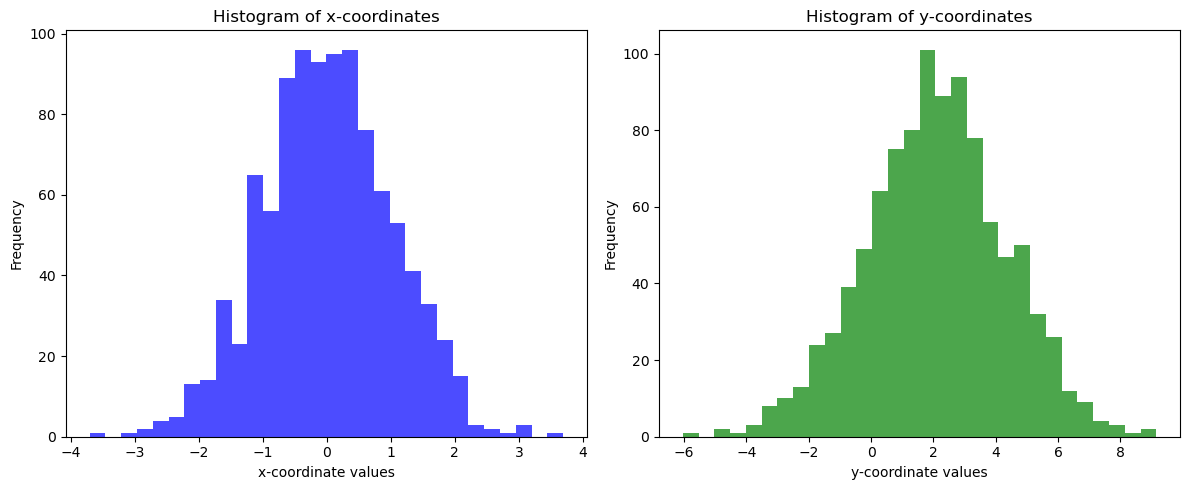
\includegraphics[width=\linewidth]{/Users/luninghao/Documents/Study/CS & DS/CSCI-SHU 360 Machine Learning/Homework/HW1/4.2.png}
    % \caption{}
    % \label{fig: 6.1} 
\end{figure}

\subsection*{4.3 Solution:}
From the histogam, we can tell that the x-coordinates of X samples are from some Gaussian distribution.\\
The mean of x-coordinates is 0.019092651459051646. The variance of x-coordinates is 1.0348564864741474. \\
We can also tell that the y-coordinates of X samples are from some Gaussian distribution.\\
The mean of x-coordinates is 2.0605238541899022. The variance of x-coordinates is 2.0605238541899022.

\newpage
\subsection*{4.4 Solution:}
\begin{figure}[h]
    \centering
    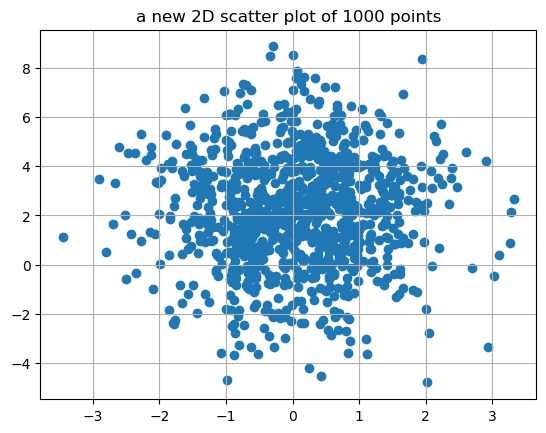
\includegraphics[width=0.4\linewidth]{/Users/luninghao/Documents/Study/CS & DS/CSCI-SHU 360 Machine Learning/Homework/HW1/4.4.png}
    % \caption{}
    % \label{fig: 6.1} 
\end{figure}

\subsubsection*{Difference:}
The original plot shows that there's a linear correlation between x-coordinates and y-coordinates, which shows that x and y are dependent and this coincides with the previous code. The new graph's circular pattern shows that there's no apparent relationship between x and y coordinates (They are independent).

\subsubsection*{What causes such difference?}
From the code in the previous section in the jupyter notebook we can see that the first plot is generated from some multivariate Gaussian distribution with a covariance between x and y coordinates so the graph they form shows a linear pattern, indicating they are correlated. While the second plot is generated from 2 independent 1D Gaussian distributions, so their graph shows a circular pattern.

% Creating a 2-column layout for 4.5 and 4.6
\begin{figure}[h]
    \centering
    \begin{minipage}{0.45\linewidth}
        \centering
        \subsection*{4.5 Solution:}
        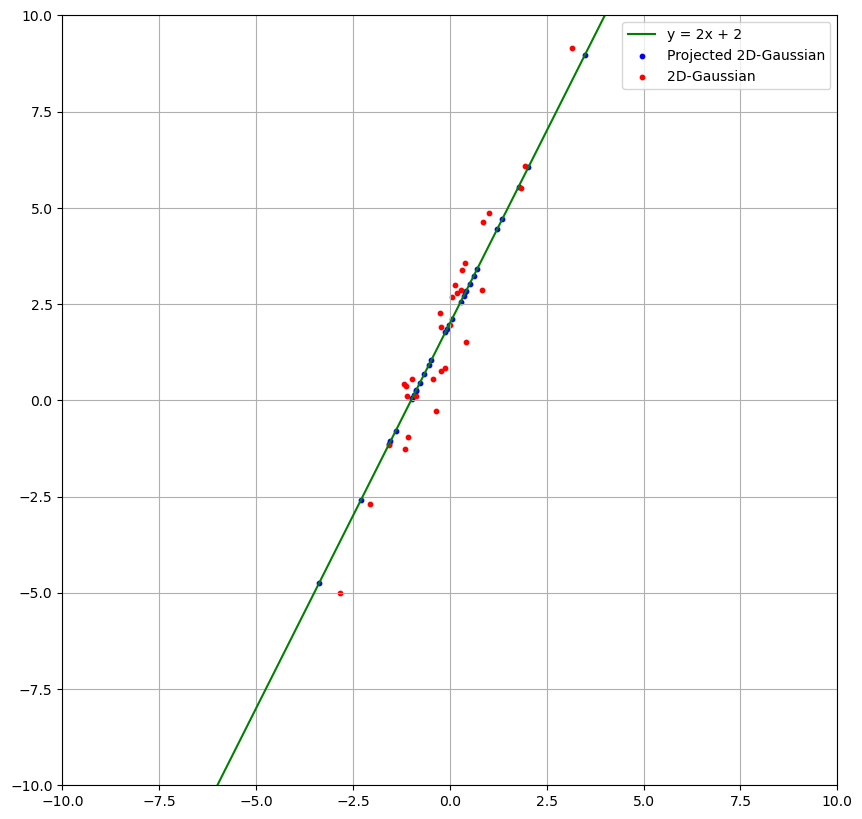
\includegraphics[width=0.9\linewidth]{/Users/luninghao/Documents/Study/CS & DS/CSCI-SHU 360 Machine Learning/Homework/HW1/4.5.png}
        % \caption{}
    \end{minipage}
    \hfill
    \begin{minipage}{0.45\linewidth}
        \centering
        \subsection*{4.6 Solution:}
        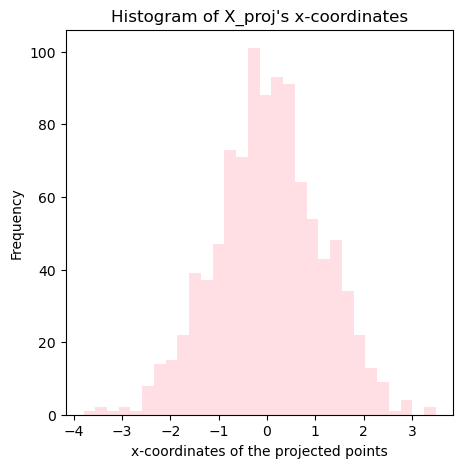
\includegraphics[width=0.9\linewidth]{/Users/luninghao/Documents/Study/CS & DS/CSCI-SHU 360 Machine Learning/Homework/HW1/4.6.png}
        % \caption{}
    \end{minipage}
\end{figure}

\subsection*{4.6 Solution: (Additional Text)}
The histogram shows that the x-coordinates of the projected points are from some Gaussian distribution. The mean of x-coordinates: 0.028028071967771222 and the variance of x-coordinates: 1.1843834728271614.





\newpage
\section*{Exercise 5}
\subsection*{5.1 Solution:}
\begin{itemize}
    \item Elements in class setosa: 50.
    \item Elements in class versicolor: 50.
    \item Elements in class virginica: 50.
\end{itemize}

\subsection*{5.2 Solution:}
The accuracy is 100 \%. This result doesn't give me useful information because this model is trained on the whole dataset, which means it actually memorizes this dataset and this leads to overfitting. The model will assign each 
data point to itself when we use the same data set for training and testing when k = 1, resulting in accuracy = 100 \%. But this doesn't mean this model will perform well on new data. As a result, when we train the model, we should split the dataset so that we can test its generalization ability.

\subsection*{5.3 Solution:}
\begin{figure}[h]
    \centering
    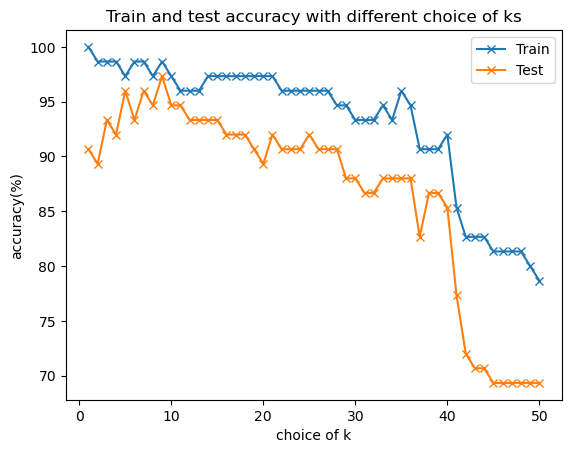
\includegraphics[width=0.65\linewidth]{/Users/luninghao/Documents/Study/CS & DS/CSCI-SHU 360 Machine Learning/Homework/HW1/5.3.png}
    % \caption{}
    % \label{fig: 6.1} 
\end{figure}
According to the graph above, when k = 9, the training accuracy and testing accuracy become most closest and this means the model has the best ability to generalize when k = 9, indicating the best possible performance.  So 9 is the optimal k. 

\subsection*{5.4 Solution:}
The predicted class is: versicolor.







\newpage
\section*{Exercise 6}
\subsection*{6.1 Solution:}
\begin{figure}[h]
    \centering
    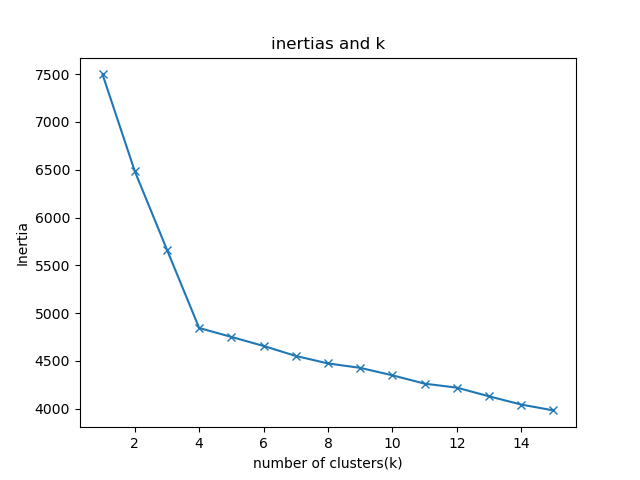
\includegraphics[width=0.65\linewidth]{/Users/luninghao/Documents/Study/CS & DS/CSCI-SHU 360 Machine Learning/Homework/HW1/6.1.png}
    % \caption{}
    % \label{fig: 6.1} 
\end{figure}
Based on this plot, the elbow point indicates that 4 clusters should be used for this data.

\subsection*{6.2 Solution:}
25 observations are placed in each cluster, the value of inertia is 4844.925817623823.
\subsection*{6.3 Solution:}
\begin{figure}[h]
    \centering
    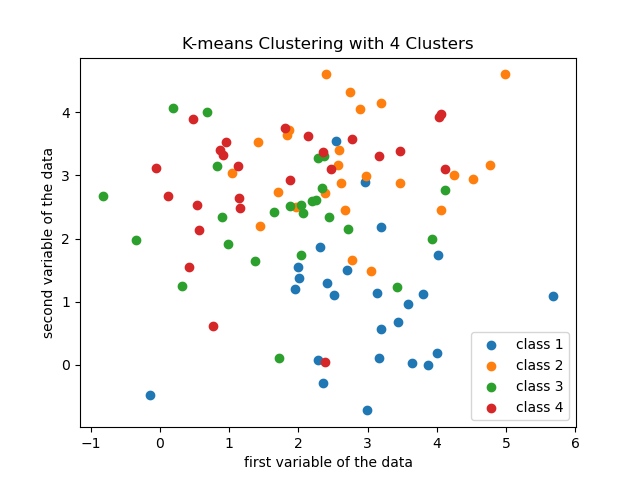
\includegraphics[width=0.65\linewidth]{/Users/luninghao/Documents/Study/CS & DS/CSCI-SHU 360 Machine Learning/Homework/HW1/6.3.png}
    % \caption{}
    % \label{fig: 6.3} 
\end{figure}
Based on this plot, I cannot conclude that 4 is good for the number of centers since graph based on the first and second variable does not separate the data points. The data points on the graph mixed together. Maybe we need to choose other variables to better visualize.
\end{document}